%===================================== CHAP 4 =================================

\chapter{Neural Linear Bayesian Regression Model}\label{ch:bdqn}

A drawback of the methods discussed in chapter \ref{ch:linear} is that they are all linear models. These cannot perform well in environments with complex non-linear relationships between state-action pairs and Q-values without significant feature engineering. Recent developments in the RL field focus on deep RL where neural networks are used to encode these relationships have allowed successful results on complex games\citep{mnih_2015, mnih_2016,silver_2017}. As such it it would be beneficial to be able to combine the methods from chapter \ref{ch:linear} with more complex models. This chapter attempts this and tests the new model on multiple complex environments with comparisons to other popular deep RL methods.

\section{Combining Bayesian Q-learning with Neural Networks}

\subsection{Neural Linear Model}

Without significant feature engineering a linear model cannot generalize to more complex non-linear relationships between state-action pairs and their Q-values. However using bayesian methods with non-linear models can be difficult and computationally heavy. \cite{carlos_2018} compared a large array of bayesian models on a set of bandit environments. They found that accurate complex models often performed worse than simpler approximate methods. The suggested reason for this is that complex models require more data and training to achieve reasonable variance estimates. Since RL is an online task this can lead to miscalibrated variance early on in the training process that leads to worse results.

Empirically \cite{carlos_2018} finds what they coin the neural linear model to work best. The model consists of using a neural network as a basis function that is used as the covariates to a linear bayesian regression model. This is equivalent to rewriting the regression task to 

\begin{equation*}
	Q = \phi(X)\beta + \varepsilon \quad \text{where} \quad \varepsilon \sim N(0,\sigma^2)
\end{equation*}

where $\phi(X)$ is the neural networks output given an input $X$. The error in the bayesian regressions point estimate is backpropagated through the neural network to learn a useful basis function. Note that this means the bayesian regression no longer incorporates all the model uncerainty since the above assumes no uncertainty in the $\phi(X)$ encoding. \cite{carlos_2018} suggests that this assumption is counteracted by the models stable uncertainty estimates.

This setup allows the application of the methods discussed in chapter \ref{ch:linear} in more complex environments.

\subsection{Bayesian DQN Models}

Based on the results of \cite{carlos_2018} this thesis attempts to combine neural networks and the BNIG model through a neural linear setup. To start off a summary of the architecture used in \cite{azziz_2018}, called the BDQN, is provided. This is used as a base which will modified to fit with the BNIG model and thus allow for better variance propagation.

The BDQN architecture starts with the same architecture as the standard DQN architecture\citep{mnih_2015}. The final layer of a DQN is a linear layer which means it can be replaced by any linear model. \cite{azziz_2018} replaces this with a BN model and uses the MAP target for both without considering the possibility of sampling the target. The neural network is trained using the loss function

\begin{equation*}
	\theta = \theta - \alpha\nabla_\theta\big(Q_t - [\mu_n^T\phi_\theta(x_t)]\big)^2.
\end{equation*}

 The only difference to a regular neural network is that the networks output estimate is replaced by the MAP estimate of $\beta$. One could replace the MAP estimate by samples from the posterior $Q$. However as the network does not consider the variance of the target using the MAP leads to a lower computational cost and a more stable loss signal. The pseudocode for this update is

\begin{algorithm}[H] 
    \caption{BDQN Network Training} 
    \label{alg:BDQN_train} 
        \If{$t \; \textbf{mod} \; T_{train}$ == $0$}{ 
            Sample random minibatch of transitions $(s_j, a_j, r_j, s_{j+1})$ from $\mathcal{D}$ \\ 
            $a' = \argmax_a \big[\phi(s_t)\mu_a\big]$ for each transition \\ 
            Set $y_j = \begin{cases} 
                r_j \quad \text{for terminal} \quad s_{j+1}\\ 
                r_j + \gamma\phi^*(s_t, a')\mu^*_{a'} \quad \text{else} 
            \end{cases}$ \\ 
            Optimize the network weights over the Huber loss (equation \ref{eq:huber_loss}) 
        } 
\end{algorithm}

The BN model is trained using the BN posterior updates described in equation \ref{eq:known_noise_posterior_update}. Since the BN model does keep track of variance one could consider using a sample targert rather than the MAP target in this case. However it has already been shown that in the linear case using a sampled target over a MAP target has no effect on the final estimate as it does not propagate uncerainty.

These two training processes do not have to happen sequentially. In \cite{azziz_2018} the neural network is updated as frequently as in the original DQN implementation, while the bayesian regression trained from scratch every 10,000 steps on either 100,000 datapoints or the entire replay buffer if it contains less. This is done to handle the non-stationarity of the task. 

\subsection{From BDQN to BNIG DQN}

The downside retraining the bayesian regression is that this is computational heavy, especially considering that the final layer in the neural network consists of 512 neurons, meaning the update requires matrix arithmetic with a 512 by 512 matrix. On top of this using a BNIG model requires the target Q-values to be sampled from the posterior. This means every 10,000 steps 100,000 new samples must be drawn which requires a new set of matrix arithmetic of the same magnitude. Instead this thesis considers the exponential forgetting method. However implementing this requires some extra considerations to ensure that the model remains stable.

Recall that the classic DQN has one online network that is updated each training step and one target network that is updated occasionally to match the online network. \cite{mnih_2013} found that using this target network to calculate the regression target helped stabilize the algorithm.

With exponential forgetting the bayesian regression is trained continuously. However, using the online bayesian regression method to calculate targets based on the output from the target network will lead to instability. The regression model can train on thousands of datapoints from the online network between network syncs. Using different network encodings for the target and prediction with the same bayesian regression will lead to a different results which will increase the loss. An increased loss leads to larger network changes which amplifies the effect leading to instability.

To deal with this issue the same online-target structure used for the networks is used for the regression models. Two bayesian regression models are created, one online and one target. The target model is used to calculate the target action-values while the online model is used for decision making. The target model is then updated to the parameters of the online model when the target network is updated. This decreases the loss and resulted in a stable network. The pseudocode for this update is seen in algorithm \ref{alg:bnig_train}. Note that the $^*$ notation denotes values from the target parameters and $\varepsilon_a$ is a sample from $N(0,\sigma^2_a)$.

\begin{algorithm}[H]
    \caption{BNIG training}
    \label{alg:bnig_train}
        \If{$t \; \textbf{mod} \; \textit{batch size} == 0$}{
            Sample random minibatch of transitions $(s_j, a_j, r_j, s_{j+1})$ from $\mathcal{D}$ \\
            Sample $\beta_a, \sigma_a$ for $a\in \mathcal{A}$ for each transition\\
            $a' = \argmax_a \bigg(\phi(s_t)\beta_a + \varepsilon_a\bigg)$ for each transition \\
            Sample $\beta^*_{a'}, \sigma^*_{a'}$ for $a'$ in each transition \\
            Set $y_j = \begin{cases}
                r_j \quad \text{for terminal} \quad s_{j+1}\\
                r_j + \gamma\bigg(\phi^*(s_t, a')\beta^*_{a'} + \varepsilon^*_{a'}\bigg)\quad \text{else}
            \end{cases}$ \\
            Update BNIG model parameters using posterior update equation \ref{eq:unknown_noise_posterior_update}
        }
\end{algorithm}

With this approach the only required change to transform the BDQN setup to a BNIG method is to swap out the BN model used in the BDQN with the BNIG model and sample action-values from the posterior for both the online and target models. The resulting algorithm is summarized in the pseudocode below.

\begin{algorithm}[H]
    \caption{BNIG DQN}
    Initialize variables according to algorithm \ref{alg:bnig_init}\\
    \For{episode = 1, M}{
        Initialize environment\\
        $s_1 = $ initial environment state\\
        
        Sample $\beta_a, \sigma_a$ for $a\in \mathcal{A}$\\
        \For{t=1, T}{
            $a_t = \argmax_a \bigg(\phi(s_t)\beta_a + \varepsilon_a$\bigg) \\
            Execute action $a_t$ and observe reward $r_t$ and state $s_{t+1}$ \\
            Store transition $(s_t, a_t, r_t, s_{t+1})$ in $\mathcal{D}$\\
            Train online network using algorithm \ref{alg:dqn_train}\\
            Train online model using algorithm \ref{alg:bnig_train} \\
            \If{$t \; \textbf{mod} \; T_{sync}$ == $0$}{
                Set target network weights to online network weights\\
                Set target BNIG parameters to online BNIG parameters.
            }
        }
    }
\end{algorithm}

Here $T_{sync}$ is a hyperparameter that defines how often to sync the online and target network and model. Once again $\varepsilon_a$ represents a sample from $N(0,\sigma^2_a)$. The initialization process in algorithm \ref{alg:bnig_init} sets up the models, networks and experience buffer required.

\begin{algorithm}[H]
    \caption{BNIG DQN Initialization}
    \label{alg:bnig_init}
    Initialize experience buffer $\mathcal{D}$ with capacity $N$\\
    Initialize neural network $\phi$ with random weights $\theta$\\
    Initialize target neural network $\phi*$ with weights $\theta^*=\theta$\\
    Initialize $|\mathcal{A}|$ BNIG models with priors $\mu_a = zeros(p,1)$, $\Sigma_a = diag(p,p)$, $\alpha_a = 1$, $\beta_a = 0.01$
    Initialize target BNIG models with priors $\mu^*_a = \mu^*_a$, $\Sigma^*_a = \Sigma^*_a$, $\alpha^*_a = \alpha^*_a$, $\beta^*_a = \beta^*_a$.
\end{algorithm}

\section{Experiment Setup}

The rest of this chapter consists of comparing the BNIG DQN to the regular DQN on a variety of environments. There are many factors that effect how well a RL model is perceived to perform so a few precautionary steps were taken to keep comparisons as fair as possible. 

\subsection{Implementation}

To ensure a correct implementation of the DQN and a fair comparison to the BNIG DQN the python package Dopamine\citep{castro_18} was used. This package contains an implementation of a DQN that matches the baselines of the \cite{mnih_2015}. The BNIG DQN was implemented on top of this DQN implementation.

\subsection{Hyperparameter Tuning}

The hyperparameters used in Deep RL can have large effects on the performance of the methods. Due to this it is important not to bias the results towards a model due to tuning hyperparameters more for one model than the other. 

To avoid this and due to computational constraints the DQN hyperparameters were taken from the Dopamine package. For the corridor environment, which is not included in Dopamine, the hyperparameters were taken from the supplemental material provided for \cite{osband_2018}. The BNIG DQN hyperparameters that are not contained in the DQN, such as the priors, were set to the corresponding values from the linear example. The only exception to this was the forgetting rate, which was decreased on all environments apart from cartpole due to the longer episodes of these environments. This approach meant that if the results were to be biased it would most likely be towards the DQN.

However a quick run through on the different environments resulted in the BNIG DQN failing on all environments. The smallest change found that lead to successful runs using the BNIG DQN was to increase from a 1-step update to a 3-step update. This change is known to give improvements to the DQN method \citep{hessel_2017} so the DQN hyperparameters were also changed to match this. To ensure that this was not detrimental to the DQN model performance all environments have been run using both the 1-step and 3-step DQN where the 3-step outperformed the 1-step across all environments.

A detailed overview of the hyperparameters per environment is provided in the appendix.

\subsection{Model Evaluation}

The comparison of the two methods is based on their performance on the environment relative to the number of samples it has trained on. To fairly compare the methods during training the experiments the results are gathered from an evaluation stage. The evaluation stage is run every time one wants to measure the performance of the method and consists of calculating the average total reward over a few episodes.

In this evaluation phase the model and network are not trained. The DQN agent acts greedily with respect to the DQN output, in other words with $\varepsilon=0$. The BNIG DQN acts greedily with respect to it's MAP estimate. This means it acts based on the mean $\beta$ values and no noise.

\section{BNIG DQN Results}

\subsection{Corridor}

% However as an additional challenge half of states the actions are swapped, meaning action 1 moves left and action 0 moves right. Note that this is still a stationary environment. The swapped states are randomly chosen the first time the environment is initialized and stay the same throughout the training process.

The first environment test is the same environment as the corridor environment introduced in chapter \ref{ch:linear}. Due to computational constraints a chain length versus time to learn figure, like figure \ref{fig:linear_corridor}, was not possible. Instead single seeds were tested on different chain lengths of increasing size until one of the methods started failing. This occurred at corridor length 10. Each model was then run 10 times on the length 10 corridor with results presented in figure \ref{fig:nn_corridor}.

\begin{figure}[H]
    \centering
    \subfloat[DQN]{
        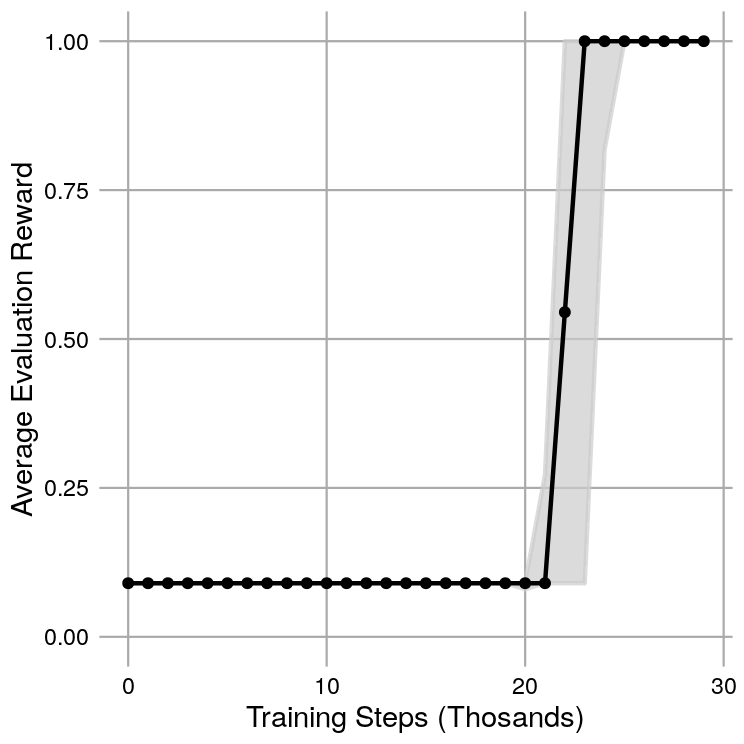
\includegraphics[scale=0.5]{DQNCorridor.png}
    }
    \subfloat[BNIG DQN]{
        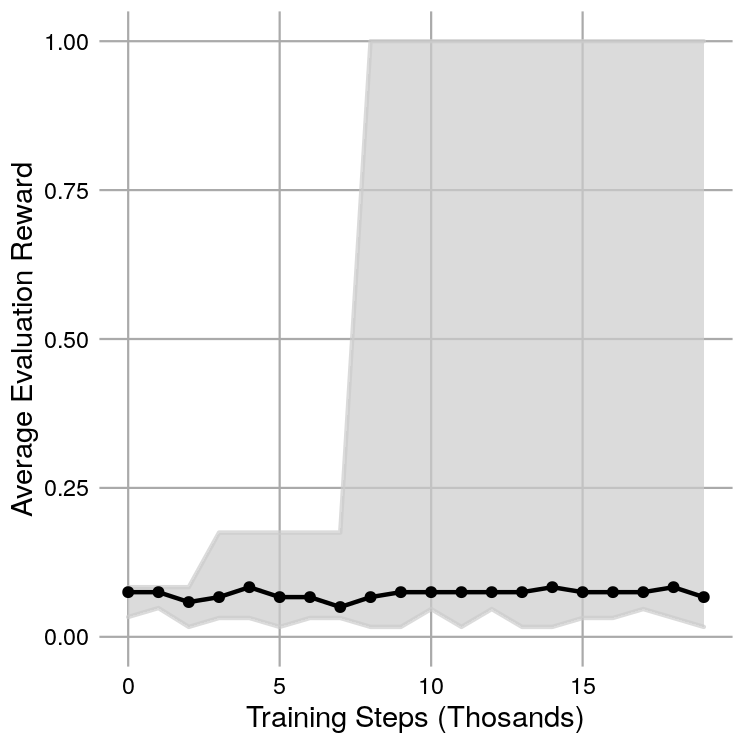
\includegraphics[scale=0.5]{BDQNCorridor.png}
    }
    \caption{\textbf{DQN and BNIG DQN Performance on Corridor}: Plots show the median performance over 10 different attempts. The shaded area covers 80\% of the total reward over all attempts.}
    \label{fig:nn_corridor}
\end{figure}

In contrast to the linear case the $\varepsilon$-greedy DQN method outperforms the BNIG DQN. In fact the BNIG DQN fails to find the correct policy across any seed (figure \ref{fig:nn_per_corridor}).


\subsection{Cartpole}

The environment considered is a classic toy example called cartpole. The environment was first proposed in \cite{barto_sutton_1983} and is available through the Open AI gym environment \citep{brockman_2016}.

\begin{figure}[H]
    \centering
    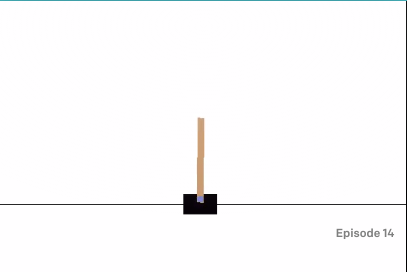
\includegraphics[scale=0.5, trim={10px, 10px, 10px, 10px},clip]{cartpole.png}
    \caption{\textbf{Cartpole Environment} The pole is in brown and the cart in black. \citep{gym_docs}}
    \label{fig:cartpole}
\end{figure}

The task, seen in figure \ref{fig:cartpole}, consists of balancing a pole on top of a cart. If the pole falls more than 15 degrees from the upright position or if the cart goes too far (2.4 units from the center) to the left or right the game is terminated. Otherwise the game is terminated after 500 timesteps and every timestep a reward of $+1$ is received. There are two actions, the cart can be pushed to the left or to the right at every timestep. There are 4 input variables that define the state: the pole angle from vertical, the position of the cart and the derivative of both variables. 

The environment implementation from OpenAI Gym was used \citep{brockman_2016}. Each method was run for 50,000 steps with 10 different seeds and every 1000 steps an evaluation phase is run over 1000 steps. The results are summarized in figure \ref{fig:nn_cartpole}.

\begin{figure}[H]
    \centering
    \subfloat[DQN]{
        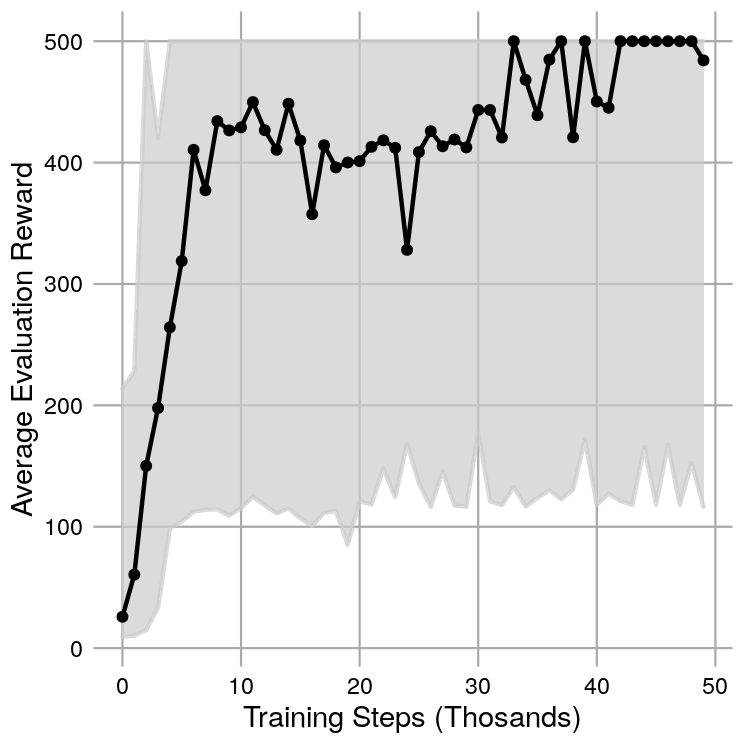
\includegraphics[scale=0.5]{DQNCartpole.png}
    }
    \subfloat[BNIG DQN]{
        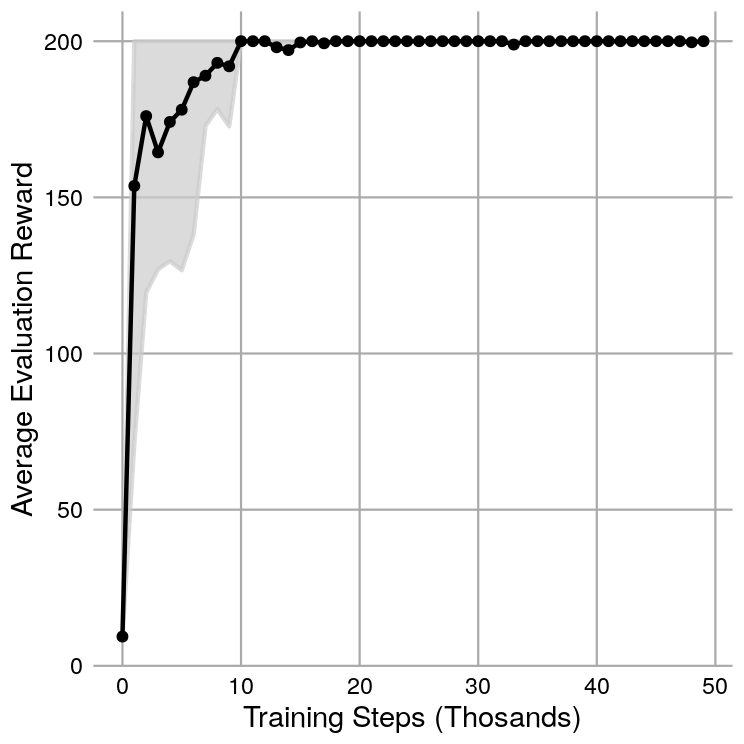
\includegraphics[scale=0.5]{BDQNCartpole.png}
    }
    \caption{\textbf{DQN and BNIG DQN Performance on Cartpole}: Plots show the median performance over 10 different attempts. The shaded area covers 80\% of the total reward over all attempts.}
    \label{fig:nn_cartpole}
\end{figure}

A policy that does not balance the pole lasts about 10 to 20 frames which is equivalent to a reward of 10 to 20. Figure \ref{fig:nn_cartpole} shows both methods are able to find successful balancing policy. However, while the max performance of the DQN matches the BNIG DQN, the latter acheives much more stable results. Breaking down the results per seeds (figure \ref{fig:nn_per_cartpole}) one can see that the spread is caused by the instability of DQN after having found an optimal policy in some attempts and failing to find the optimal policy in others. The BNIG BDQN however always finds the optimal policy however can face some deterioration in performance towards the end of the experiment. 

\subsection{Acrobot}

Another common toy example is called acrobot. The experiment is first described in \cite{hauser_1990} and put into an RL context in \cite{sutton_1996}. The environment, seen in figure \ref{fig:acrobot}, represents a vertically hanging 2D, two joint robot arm. The first joint's position is fixed to the origin while the second join has an actuator. This actuator can apply torque to the second joint. The arm starts hanging downwards under the origin. The goal is to balance the force of gravity, the actuators output and the momentum of the arm to swing the end of the arm over a line above the origin. Achieving this terminates the episode. A reward of $-1$ is given each timestep. The state input is

$$
[\cos(\theta_1), \sin(\theta_1), \cos(\theta_2), \sin(\theta_2), \dot{\theta}_1, \dot{\theta}_2]
$$

where $\theta_1$ is the angle of the first joint and $\theta_2$ is the angle of the second joint relative to the first. The agent can apply -1, 0 and +1 torque to the second joint.

\begin{figure}[H]
    \centering
    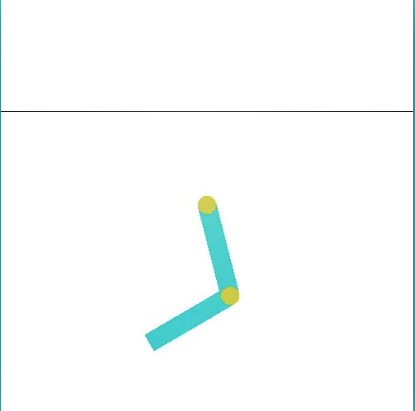
\includegraphics[scale=0.4, trim={10px, 10px, 10px, 10px},clip]{acrobot.png}
    \caption{\textbf{Acrobot Environment}: A still frame from the OpenAI acrobot implementation. The joints are marked in yellow, the arms in blue and the line represents the threshold. Image from \cite{gym_docs}}
    \label{fig:acrobot}
\end{figure}

The environment implementation from OpenAI Gym was used \citep{brockman_2016}. Each method was run for 50,000 steps with 10 different seeds and every 1000 steps an evaluation phase is run over 1000 steps. The environment and performance is seen in figure \ref{fig:nn_pong} 

\begin{figure}[H]
    \centering
    \subfloat[DQN]{
        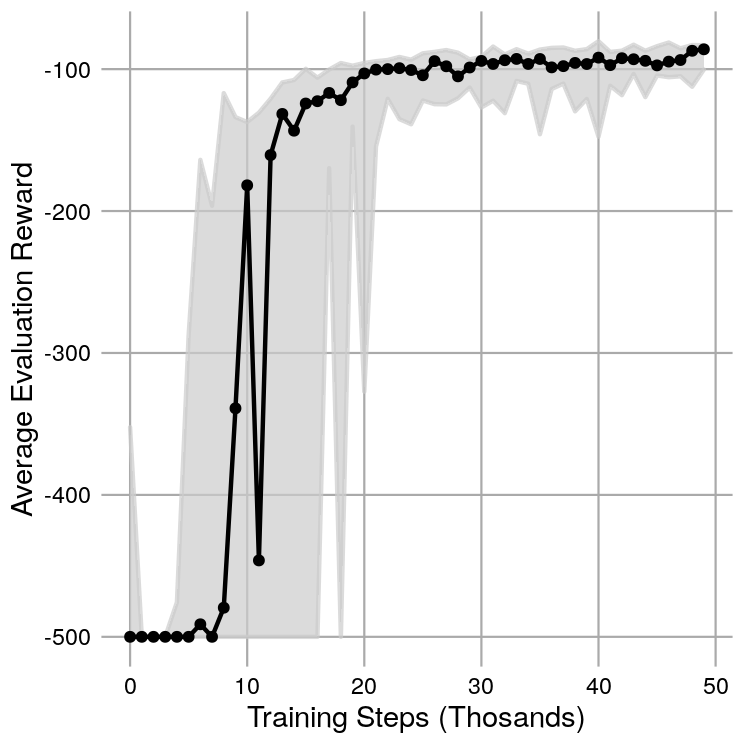
\includegraphics[scale=0.5]{DQNAcrobot.png}
    }
    \subfloat[BNIG DQN]{
        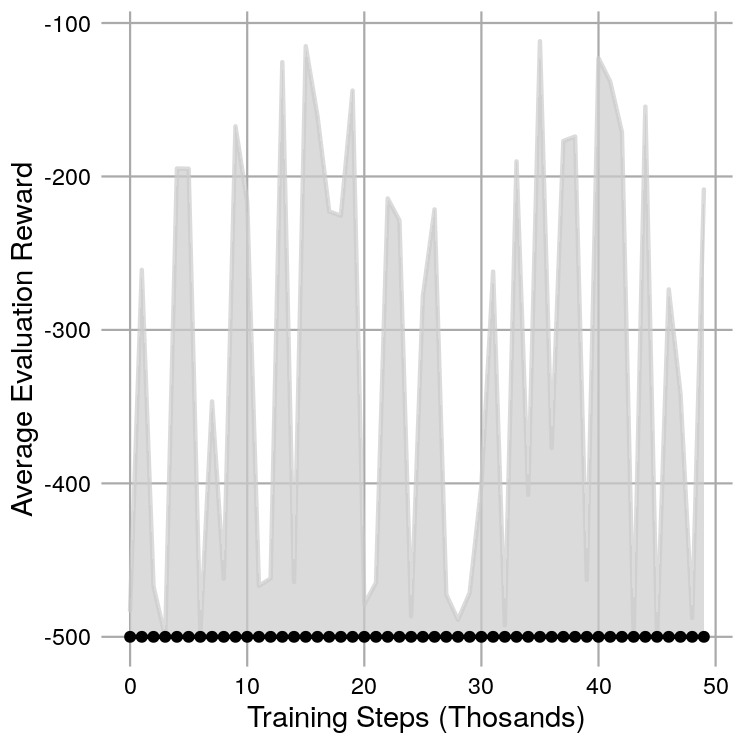
\includegraphics[scale=0.5]{BDQNAcrobot.png}
    }
    \caption{\textbf{DQN and BNIG DQN Performance on Acrobot}: Plots show the median performance over 10 different attempts. The shaded area covers 80\% of the total reward over all attempts.}
    \label{fig:nn_acrobot}
\end{figure}

A score above -500 indicates the agent was able to lift the robot arm over the required threshold. Figure \ref{fig:nn_acrobot} shows both agents are occasionally able to do this. However, while the DQN model find a stable policy leading to an average reward of -100, the BDQN struggles to stay above -500. A deeper look into the per seed results (figure \ref{fig:nn_per_acrobot}) shows that the BDQN acheives an average reward of around -100 every seed. However, it is unable to keep this policy over more than two iterations before falling to a -500 reward again. There are many possible reasons. It can be caused by a too high learning rate, a miscalibrated exponential memory or a miscalibrated target update time period to a name a few.

\subsection{Atari}

A standard benchmark in the deep RL field is a large set of atari 2600 games called the Arcade Learning Environment(ALE) introduced in \cite{bellemare_13}. Papers presenting new methods in this field generally tested for 200 million frames on 40-50 of these games, such as in \cite{mnih_2015}, \cite{mnih_2016} and \cite{donoghue_2017}. All environments must be learned based purely on the image input from the game. Due to the difficulty of the games and the large networks required the learning process is heavy to run, often taking close to a week on a GPU per game. Due to limited compute the BNIG DQN was tested once a subset of these games. The results were compared to 5 seeds of DQN runs that can be found in the Dopamine package. Both methods use all the same hyperparameters with the exception of the update horizon, which was set to 5 for the BNIG DQN. This is known to increase the performance of the DQN, so the results are not a completely fair comparison.

\subsubsection{Pong}

Pong is one of the simpler environment in the ALE with superhuman performance acheived already in 2013\citep{mnih_2013}. The game consits of two paddles and a ball. The aim of the game its to hit the ball past the other players paddle which results in a +1 reward. If the other player hits the ball past the agents paddle it receives a -1 reward. 

\begin{figure}[H]
    \subfloat[Environment]{
        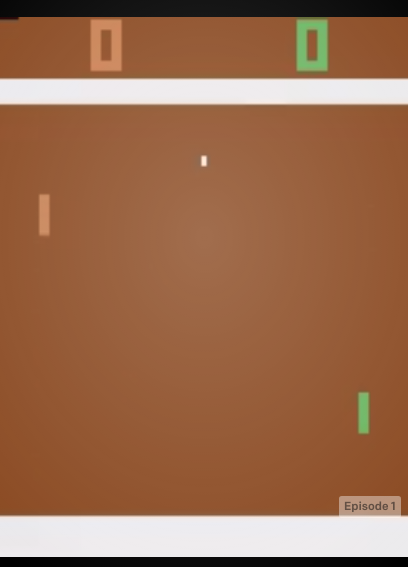
\includegraphics[scale=0.4, trim={10px, 50px, 10px, 20px},clip]{pong.png}
    }
    \subfloat[Performance]{
        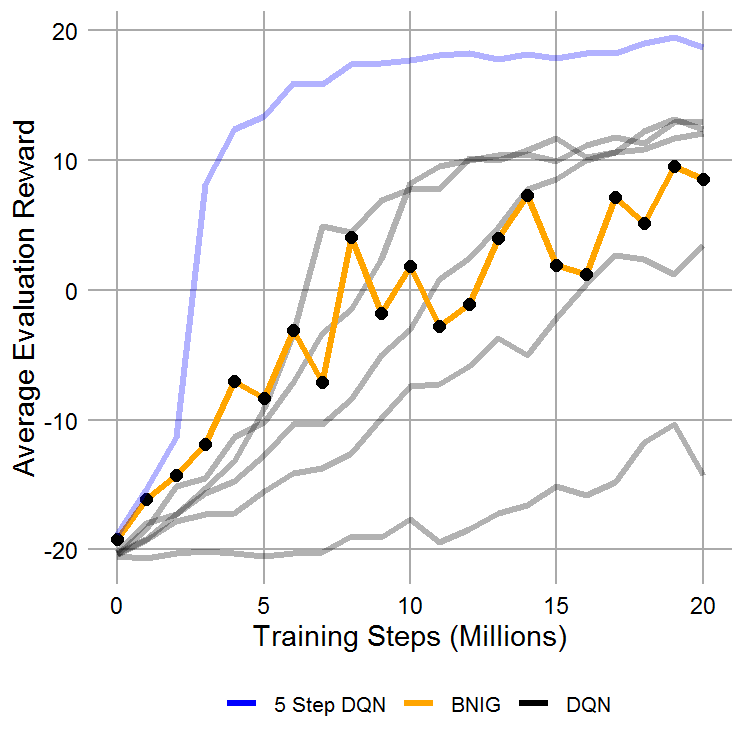
\includegraphics[scale=0.5]{BDQNPong.png}
    }
    \caption{\textbf{Pong environment results}: \textbf{(a)} shows an input state of the pong environment\citep{gym_docs}. The green panel is the agent and the ball is in white. \textbf{(b)} compares the BDQN performance in orange to the 5 DQN runs provided in Dopamine.}
    \label{fig:nn_pong}
\end{figure}

BNIG started off well, with better evaluation performance than all DQN seeds for the first 5 iterations. From there on out the improvements decrease and the evaluation becomes more unstable. After 35 million steps BNIG has similar to slightly worse results than the DQN. Since this test only compares 1 seed to 5 seeds there is not enough data to confidently evaluate the performance but the results indicate the performance is similar to the DQN albeit more unstable. Taking into consideration that BNIG is using a 5-step update, which should improve performance, the underlying BNIG method seems to actually worse than DQN on this game.

\subsection{Stabilizing Variance}

Due to the stability issues seen on acrobot and pong an attempt was made at tuning the hyperparameters of the BNIG model to see if this could get better results. A deeper look at the development of the model parameters for the acrobot environment showed that the scale parameters $b_a$ become increasingly unstable as seen in figure \ref{fig:scale_stability}a. Multiple attempts were made at controlling this increase but the only successful result came from adjusting the initial inverse gamma distribution towards a lower variance output. The reasoning for this will be discussed in chapter \ref{ch:disc}. Note that the statical arguments that follow aren't especially strong originating from the fact that exponential forgetting does not have a strong statistical fundament. The goal of this subsection is purely to show the potential of the BNIG methods given a more stable posterior update.  %increasing the inverse gamma scale prior $a_a$.

\subsubsection{Low Varaince Prior}

One way of decreasing the variance estimate is to adjust the priors of the distribution towards a lower mean inverse gamma. This can be done by either decreasing $b_a$ or increasing $a_a$. Of the two only increasing $a_a$ improved performance. The resulting improved stability can be seen in \ref{fig:scale_stability}b.

\begin{figure}[H]
    \centering
    \subfloat[Prior Scale of 1]{
        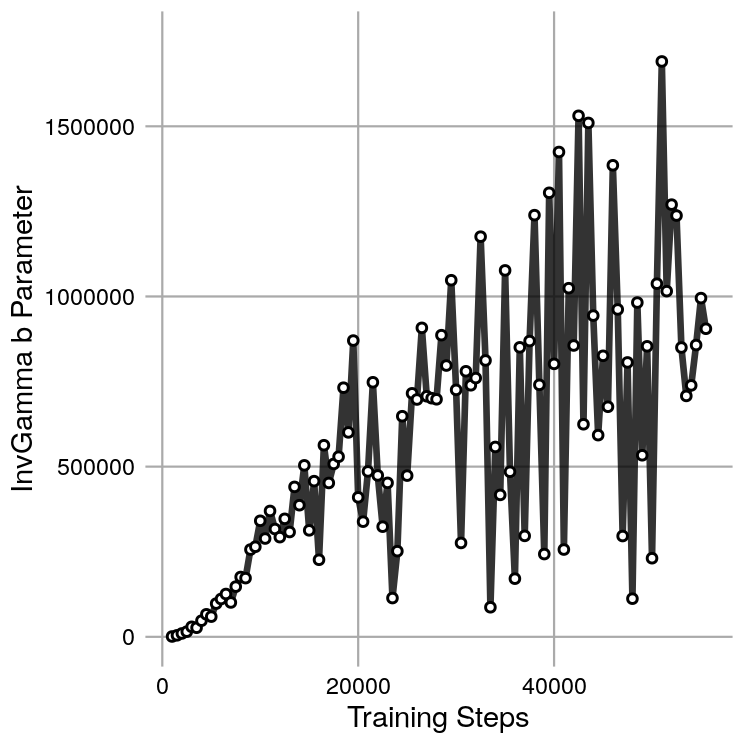
\includegraphics[scale=0.5]{BUnstable.png}
    }
    \subfloat[Prior Scale of 10,000]{
        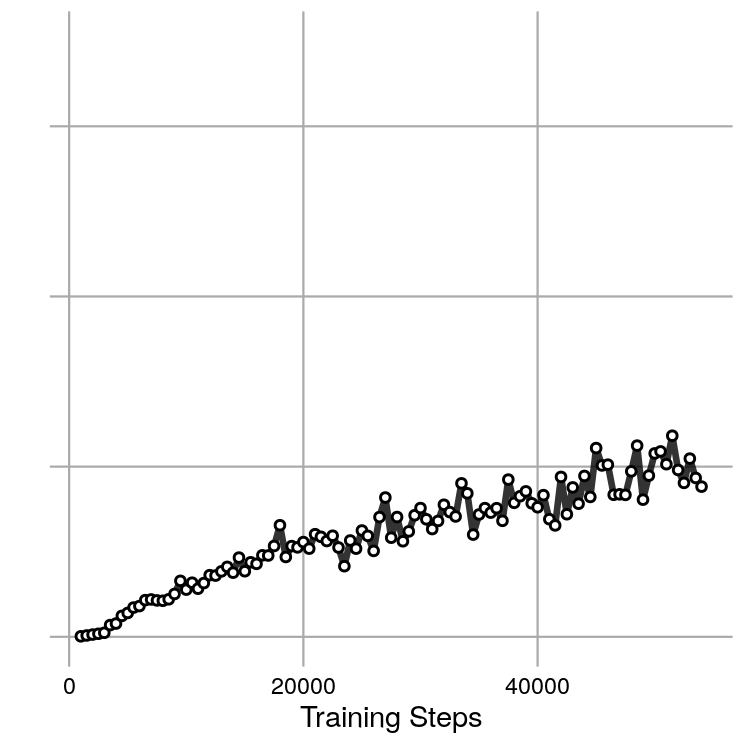
\includegraphics[scale=0.5]{BStable.png}
    }
    \caption{\textbf{Development of rate parameter given different scale priors.}}
    \label{fig:scale_stability}
\end{figure}

The effect of increasing the inverse gamma scale prior is decreasing the mean $\sigma^2$ and the variance of $\sigma^2$. This means that it pushes the posterior distribution towards a low variance $Q$-value. In general as the number of datapoints increase the resulting posterior is less and less defined by its prior. However as this method is using exponential forgetting the prior is never truly forgotten and so setting a high $a_a$ value will force a lower variance over the entire training process.

\todo Insert results for corridor and cartpole here

\begin{figure}[H] 
    \centering 
    \subfloat[Acrobot BNIG]{ 
        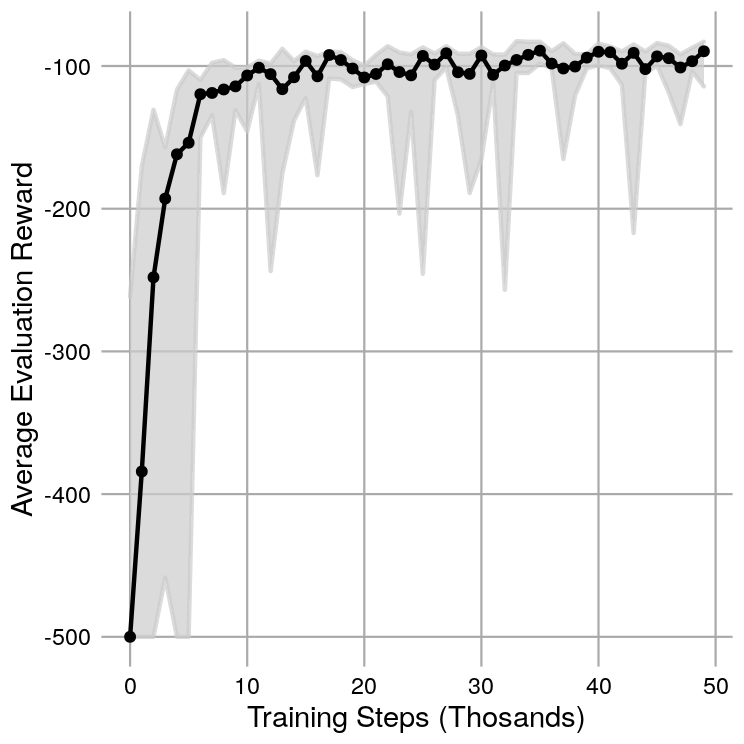
\includegraphics[scale=0.5]{AlphaBDQNAcrobot.png} 
    }
    \subfloat[Pong BNIG]{ 
        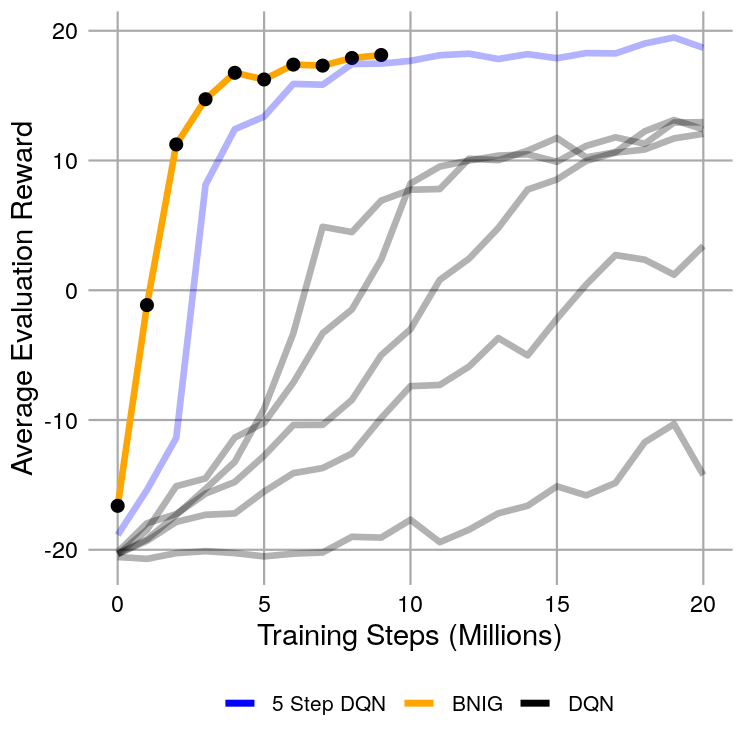
\includegraphics[scale=0.5]{BDQNPongHighAlpha.png}
    }
    \caption{\textbf{High scale prior results}} 
    \label{fig:high_scale} 
\end{figure}

The results in figure \ref{fig:high_scale} show large improvements on both pong and acrobot. The performance on cartpole is relatively unchanged while the performance on corridor seems to have become slightly worse.

\subsubsection{Data Prior}

An alternative method is to adjust the initial values for the terms used in the posterior update of the inverse gamma parameters: $y^Ty$ and $n$. Up until this point these have been set to zero representing no data. However one can set the two terms to values equivalent to the expected value of having sampled from a distribution with a given variance. Since the mean $\sigma^2$ is $\frac{b_a}{a_a-1}$ setting $y^Ty\approx n$ will give a mean $\sigma^2\approx 1$. This will be referred to as a data prior. In addition one can control for how quickly this data prior is forgotten. To do this recall that given a forgetting rate of $\alpha$ the model is trained on data as far back as $\frac{1}{1-\alpha}$ and each data point increases $n$ by $1/2$. The geometric sum of $n$ given a forgetting rate of $\alpha$ will then be $\frac{0.5}{1-\alpha}$. Therefore setting a data prior $n=y^Ty=\frac{0.5}{1-\alpha}$ will give a prior mean variance of 1 that is forgotten after $\frac{1}{1-\alpha}$ new datapoints. This can then be scaled to control the number of datapoints the data prior will have an effect. The result of doing this on the cartpole example can be seen in figure \ref{fig:scale_stability2}b.

\begin{figure}[H]
    \centering
    \subfloat[Prior Scale of 1]{
        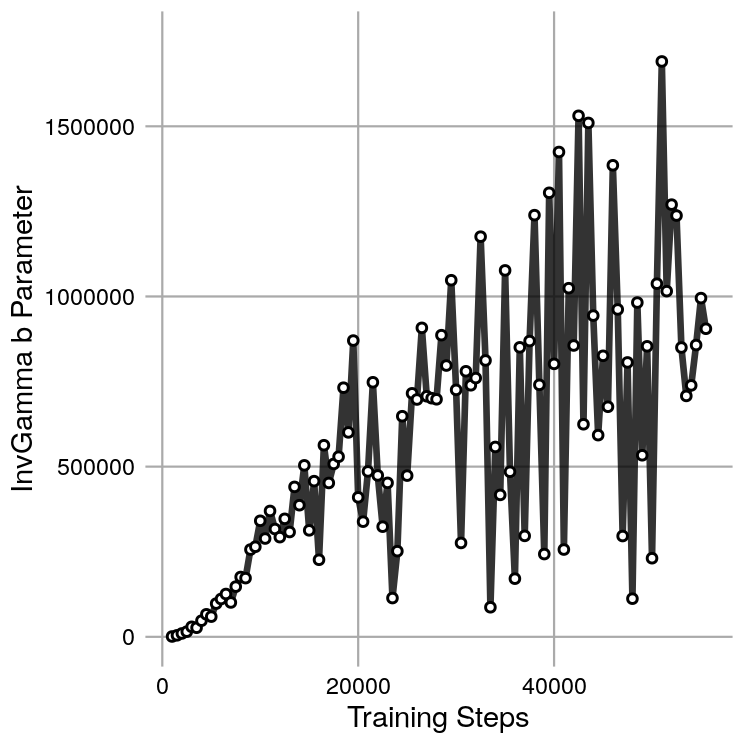
\includegraphics[scale=0.5]{BUnstable.png}
    }
    \subfloat[Data Prior]{
        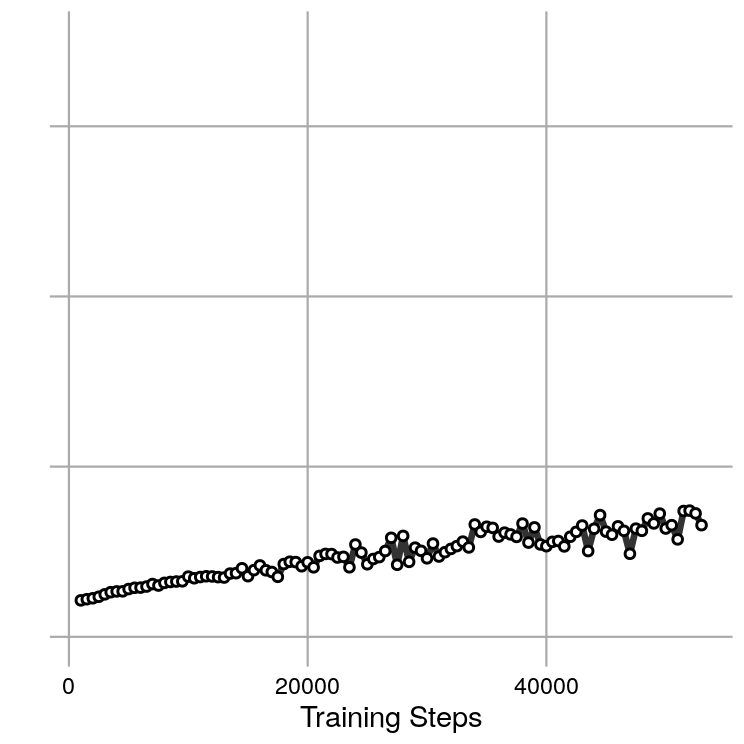
\includegraphics[scale=0.5]{BStable2.png}
    }
    \caption{\textbf{Development of rate parameter given different scale priors.}}
    \label{fig:scale_stability2}
\end{figure}

\todo Insert results for corridor, cartpole, acrobot and pong Here

\begin{figure}[H] 
    \centering 
    \subfloat[Corridor]{ 
        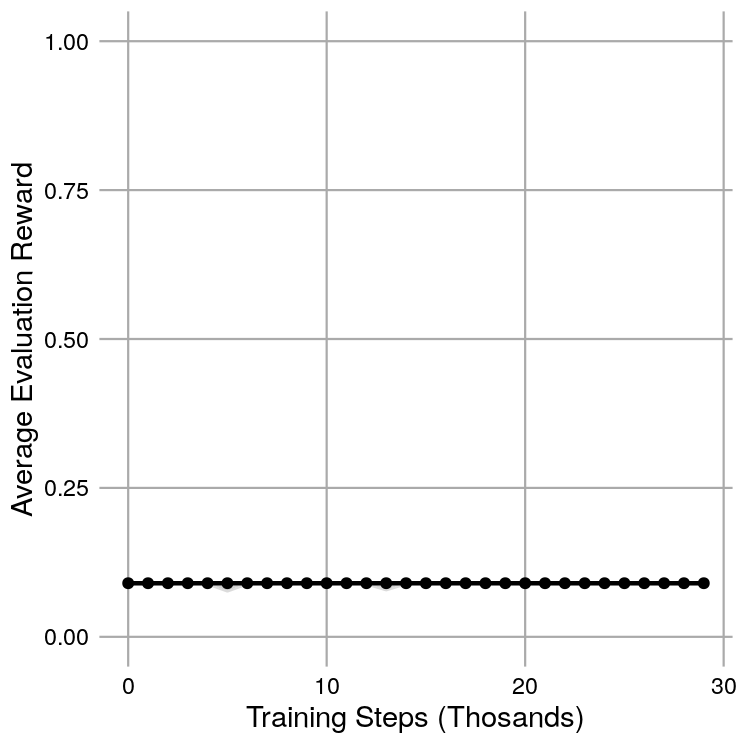
\includegraphics[scale=0.5]{RelativeBDQNCorridor.png} 
    }
    \subfloat[Cartpole]{ 
        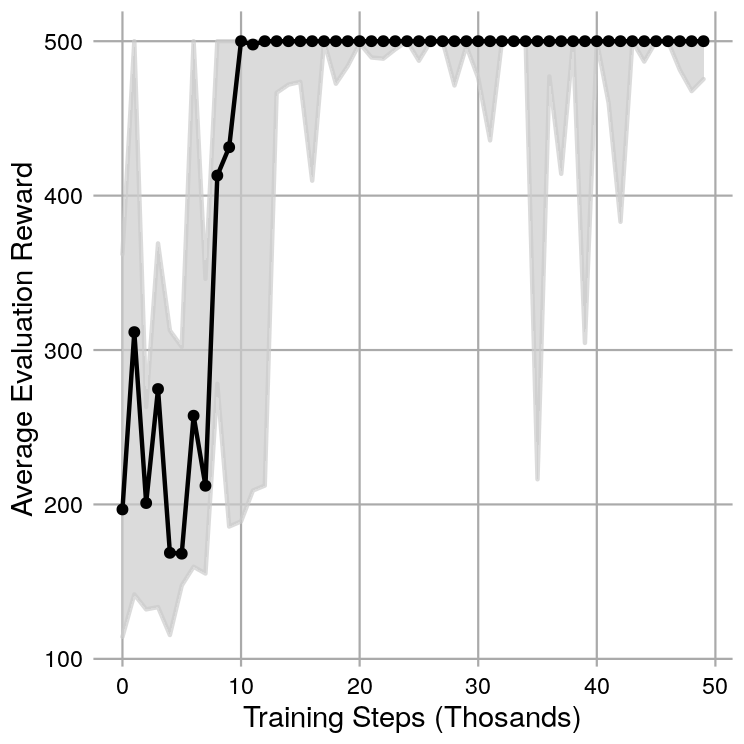
\includegraphics[scale=0.5]{RelativeBDQNCartpole.png} 
    }
    \subfloat[Acrobot]{ 
        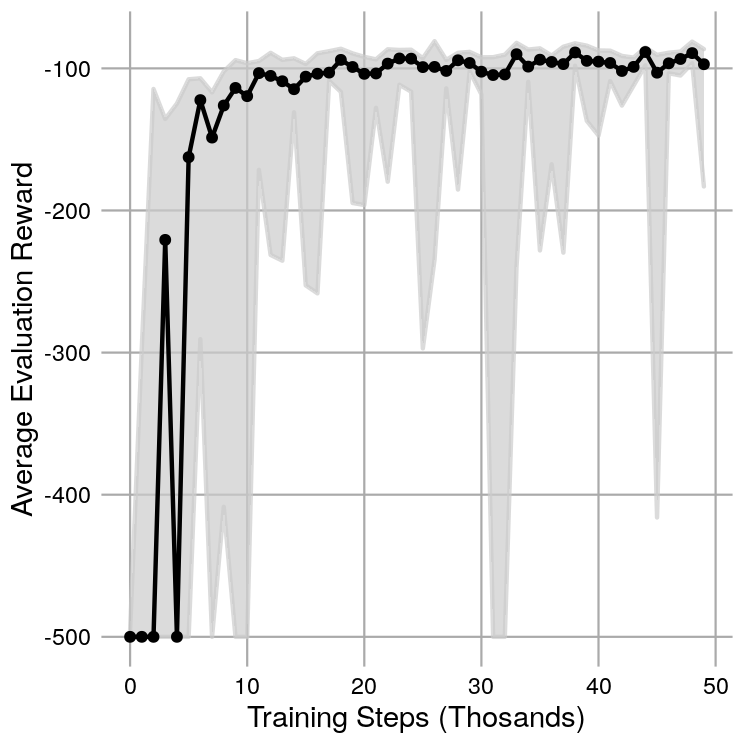
\includegraphics[scale=0.5]{RelativeBDQNAcrobot.png}
    }
    \caption{\textbf{Data prior results}} 
    \label{fig:high_scale} 
\end{figure}

\cleardoublepage